% This is samplepaper.tex, a sample chapter demonstrating the
% LLNCS macro package for Springer Computer Science proceedings;
% Version 2.20 of 2017/10/04
%
\documentclass[runningheads]{llncs}
%
\usepackage{graphicx}
\usepackage{amssymb,amsmath} 
\usepackage{hyperref}

% Used for displaying a sample figure. If possible, figure files should
% be included in EPS format.
%
% If you use the hyperref package, please uncomment the following line
% to display URLs in blue roman font according to Springer's eBook style:
% \renewcommand\UrlFont{\color{blue}\rmfamily}

\usepackage[draft,inline]{fixme}

\usepackage{pygmentex}

\FXRegisterAuthor{wh}{awh}{WH}%Wes
\FXRegisterAuthor{cn}{acn}{CN}%Chase
\FXRegisterAuthor{ep}{aep}{EP}%Eric

\newcommand{\whnt}[1]{\whnote[inline,marginclue]{\textcolor{brickred}{#1}}} 
\newcommand{\cnnt}[1]{\ydnote[inline,marginclue]{\textcolor{cobalt}{#1}}} 
\newcommand{\epnt}[1]{\epnote[inline,marginclue]{\textcolor{cobalt}{#1}}} 


\begin{document}
%
\title{Voting Theory in the Lean Theorem Prover}

%\thanks{Supported by organization x.}
%
%\titlerunning{Abbreviated paper title}
% If the paper title is too long for the running head, you can set
% an abbreviated paper title here
%
\author{First Author\inst{1}\orcidID{0000-1111-2222-3333} \and
Second Author\inst{2,3}\orcidID{1111-2222-3333-4444} \and
Third Author\inst{3}\orcidID{2222--3333-4444-5555}}
%
\authorrunning{F. Author et al.}
% First names are abbreviated in the running head.
% If there are more than two authors, 'et al.' is used.
%
\institute{Princeton University, Princeton NJ 08544, USA \and
Springer Heidelberg, Tiergartenstr. 17, 69121 Heidelberg, Germany
\email{lncs@springer.com}\\
\url{http://www.springer.com/gp/computer-science/lncs} \and
ABC Institute, Rupert-Karls-University Heidelberg, Heidelberg, Germany\\
\email{\{abc,lncs\}@uni-heidelberg.de}}
%
\maketitle              % typeset the header of the contribution
%
\begin{abstract}
There is a long tradition of fruitful interaction between logic and social choice theory. In recent years, much of this interaction has focused on computer-aided methods such as SAT solving and interactive theorem proving. In this paper, we report on the development of a framework for formalizing voting theory in the Lean theorem prover, which we have applied to verify all of the claimed properties of a recently proposed voting method. While previous  applications of interactive theorem proving to social choice (using Isabelle/HOL and Mizar) have focused on the verification of impossibility theorems, we aim to cover a variety of results ranging from impossibility theorems to the verification of properties of specific voting methods (e.g., Condorcet consistency, independence of clones, etc.). In order to formalize voting theoretic axioms concerning adding or removing candidates and voters, we work in a variable-election setting whose formalization makes use of dependent types in Lean.
% a project of formalizing definitions and theorems from voting theory in the Lean theorem prover. 

% In recent years, there has been extensive use of logical methods to study questions in social choice theory. 

%The abstract should briefly summarize the contents of the paper in
%150--250 words.

\keywords{logic and social choice theory \and voting theory \and interactive theorem proving \and Lean}
\end{abstract}
%
%
%

\section{Introduction}

\newpage

more intro...

\newpage

\section{Framework}

In this section, we define the basic objects of voting theory: profiles, social choice correspondences, etc. We first give standard set-theoretic definitions and then their type-theoretic counterparts in Lean syntax.

\subsection{Profiles}

For our set-theoretic definitions, we fix infinite sets $\mathcal{V}$ and $\mathcal{X}$ of voters and candidates, respectively. Given $X\subseteq\mathcal{X}$, let $\mathcal{B}(X)$ be the set of all binary relations on $X$. Instead of thinking of a binary relation as a set of ordered pairs, it is more convenient to think of a binary on $X$ as a function $S: X\times X \to \{0,1\}$. In fact, to better match our Lean formalization, we ``curry'' all functions with multiple arguments, transforming them into functions with single arguments that output functions. Thus, we regard a binary relation on $X$ as a function  $S:X\to \{0,1\}^X$, where $\{0,1\}^X$ is the set of functions from $X$ to $\{0,1\}$. For any $x\in X$, $S(x): X\to \{0,1\}$, and $S(x)(y)=1$ means that the binary relation $S$ holds of $(x,y)$. In what follows, we write `$xSy$' instead of $S(x)(y)=1$.

%\begin{definition} \textnormal{A \emph{profile} is a function $\mathbf{Q}:V\to \mathcal{B}(X)$ for some finite $V\subseteq\mathcal{V}$ and $X\subseteq\mathcal{X}$. Let $\mathsf{Prof}$ be the set of all profiles.}
%\end{definition}

\begin{definition}\label{ProfileDef} \textnormal{For $V\subseteq\mathcal{V}$ and $X\subseteq\mathcal{X}$, a \emph{$(V,X)$-profile} is a map $\mathbf{Q}:V\to \mathcal{B}(X)$. We write `$\mathbf{Q}_i$' for the relation $\mathbf{Q}(i)$. Given a $(V,X)$-profile $\mathbf{Q}$, let $V(\mathbf{Q})$ be $V$ and $X(\mathbf{Q})$  be $X$. We then define a function $\mathsf{Prof}$ that assigns to each pair $(V,X)$ of $V\subseteq\mathcal{V}$ and $X\subseteq\mathcal{X}$ the set $\mathsf{Prof}(V,X)$ of all $(V,X)$-profiles. Finally, define $\mathsf{PROF} = \bigcup_{V\subseteq\mathcal{V},X\subseteq\mathcal{X}}\mathsf{Prof}(V,X)$.}\end{definition}


%\textnormal{A \textit{profile} is a $(V,X)$-profile for some $V\subseteq\mathcal{V}$ and $X\subseteq\mathcal{X}$.}

%\textnormal{Let $\mathsf{Prof}(V,X)$ be the set of all $(V,X)$-profiles and $\mathsf{Prof}$ the set of all profiles.}

%\whnote{One problem with the above definition is that we cannot extract $X$ from $\mathbf{Q}$, because, e.g., $\mathcal{B}(X)$ may be empty.... In our previous papers, where $\mathbf{Q}(i)$ had to be a linear order, we can extract $X$ from $\mathbf{Q}$---provided there is more than one candidate. If there is only one candidate for $\mathbf{Q}$,  then we cannot extract $X$ from $\mathbf{Q}$....}



Depending on the application, one can interpret $x\mathbf{Q}_i y$ to mean either (i) that voter $i$ strictly prefers $x$ to $y$ or (ii) that voter $i$ strictly prefers $x$ to $y$ or is indifferent between $x$ and $y$. Under interpretation (i), we use `$\mathbf{P}$' for a profile; under interpretation (ii), we use `$\mathbf{R}$' for a profile.\footnote{\label{VoterNote}Approach (ii) is more general, since it allows one to distinguish between voter $i$ being \textit{indifferent} between $x$ and $y$, defined as $x\mathbf{R}_iy$ and $y\mathbf{R}_ix$, vs. $x$ and $y$ being \textit{noncomparable} for $i$, defined as \textit{neither} $x\mathbf{R}_iy$ \textit{nor} $y\mathbf{R}_ix$. When the distinction between voter indifference and noncomparability is not needed, approach (i) can be simpler.} A profile $\mathbf{Q}$ is said to be \emph{asymmetric} (\emph{transitive}, etc.) if for every $i\in V$, $\mathbf{Q}_i$ is asymmetric (transitive, etc.). Of course, asymmetric profiles only make sense under interpretation (i), whereas under interpretation (ii), profiles should be reflexive.

To translate Definition \ref{ProfileDef} into Lean, we first think of $V$ and $X$ as types, rather than sets, and then represent the function \textsf{Prof} from Definition \ref{ProfileDef} as follows:\footnote{When writing type expressions, arrows associate to the right, so, e.g., the expression  `\texttt{V $\to$ X $\to$ X $\to$ Prop}' stands for \texttt{V $\to$ (X $\to$ (X $\to$ Prop))}.}
%\begin{itemize}
%\item[] \texttt{def Prof: Type 0 $\to$ Type 0 $\to$ Type 0 := 
%\item[] \qquad\qquad\,\,\, $\lambda$ (V X : Type), V $\to$ X $\to$ X $\to$ Prop}
%\end{itemize}
\begin{itemize}
\item[] \texttt{\textcolor{blue}{def} \textcolor{orange}{Prof} : \textcolor{blue}{Type} $\to$ \textcolor{blue}{Type} $\to$ \textcolor{blue}{Type} := }\\\texttt{$\textcolor{blue}{\lambda}$ (V X : \textcolor{blue}{Type}), V $\to$ X $\to$ X $\to$ \textcolor{blue}{Prop}}
\end{itemize}
Here \textcolor{blue}{\texttt{Prop}} is a special type that here plays the role of $\{0,1\}$ in the formalization of binary relations mentioned above.  The definition states that \texttt{Prof} is a function that given two types, \texttt{V} and \texttt{X}, outputs the type \texttt{V $\to$ X $\to$ X $\to$ \textcolor{blue}{Prop}}. Because \texttt{X $\to$ X $\to$ \textcolor{blue}{Prop}} is the type of binary relations on \texttt{X}, an inhabitant of the type \texttt{V $\to$ X $\to$ X $\to$ \textcolor{blue}{Prop}} can be viewed as a $(V,X)$-profile. Thus, we may think of \texttt{Prof V X} as the type of $(V,X)$-profiles.

One of the most important kinds of information to read off from a profile is whether one candidate is majority preferred to another.

\begin{definition}\label{MajPrefDef} \textnormal{Given a profile $\mathbf{P}$ and $x,y\in X(\mathbf{P})$, we say that \textit{$x$ is majority preferred to $y$ in $\mathbf{P}$} if more voters rank $x$ above $y$ than rank $y$ above $x$.}\end{definition}

In Lean, we formalize Definition \ref{MajPrefDef} as follows:

\begin{itemize}
\item[] \texttt{\textcolor{blue}{def} \textcolor{orange}{majority\_preferred}  $\{$V X: \textcolor{blue}{Type}$\}$: Prof V X $\to$ X $\to$ X $\to$ Prop}\\ \texttt{:= \textcolor{blue}{$\lambda$} P x y,}\\
\texttt{cardinal.mk $\{$v : V // P v x y$\}$ >
cardinal.mk $\{$v : V // P v y x$\}$}
\end{itemize}
Here `\texttt{$\{$V X: \textcolor{blue}{Type}$\}$}' indicates that \texttt{V} and \texttt{X} are implicit arguments to \texttt{margin} of type \texttt{Type}. The \texttt{majority\_preferred} function takes in explicit arguments of a $(V,X)$-profile and two candidates  and returns the proposition stating that the cardinality of the set of voters who prefer \texttt{x} to \texttt{y} is greater than the cardinality of the set of voters who prefer \texttt{y} to \texttt{x}.

We often are concerned not only with whether one candidate is majority preferred to another but also, if so, what is the margin of majority preference.

\begin{definition}\label{MarginDef} \textnormal{Given a profile $\mathbf{P}$ and $x_1,x_2\in X(\mathbf{P})$, the \textit{margin of $x_1$ over $x_2$ in $\mathbf{P}$}, denoted $Margin_\mathbf{P}(x_1,x_2)$, is $|\{i\in V(\mathbf{P})\mid x_1\mathbf{P}_ix_2\}|-|\{i\in V(\mathbf{P})\mid x_2\mathbf{P}_ix_1\}|$.}
\end{definition}
\noindent In Lean, Definition \ref{MarginDef} becomes:

\begin{itemize}
\item[] \texttt{\textcolor{blue}{def} \textcolor{orange}{margin} $\{$V X: \textcolor{blue}{Type}$\}$  [fintype V] : Prof V X $\to$ X $\to$ X $\to$ $\mathbb{Z}$ := } \texttt{
    \textcolor{blue}{$\lambda$} P x$_1$ x$_2$, $\uparrow$(finset.univ.filter (\textcolor{blue}{$\lambda$} v, P v x$_1$ x$_2$)).card
        -} \\ \texttt{$\uparrow$(finset.univ.filter (\textcolor{blue}{$\lambda$} v, P v x$_2$ x$_1$)).card}
\end{itemize}
Here `\texttt{[fintype V]}' can roughly be understood as an implicit assumption that \texttt{V} is finite,\footnote{See \href{https://leanprover.github.io/reference/expressions.html\#implicit-arguments}{Section 3.3} of the Lean documentation and the Lean community page on \href{https://leanprover-community.github.io/theories/sets.html\#finite-types}{Sets and set-like objects}.} which we make so that we can perform the subtraction in the definition of margin. The \texttt{margin} function takes in explicit arguments of a $(V,X)$-profile and two candidates  and returns the margin of the first over the second; in particular, `\texttt{finset.univ.filter (\textcolor{blue}{$\lambda$} v, P v x$_1$ x$_2$)}' is syntax for constructing $\{v\in V(\mathbf{P})\mid x_1\mathbf{P}_v x_2\}$, \texttt{.card} takes the cardinality of the set (a natural number), and $\uparrow$ shifts the type from natural number to integer. 

\begin{comment}
In a profile $\mathbf{P}$, we say that $x$ is \textit{majority preferred} to $y$ if the margin of $x$ over $y$ is positive, formalized as follows:
\begin{itemize}
\item[] \texttt{\textcolor{blue}{def} \textcolor{orange}{margin\_pos} [fintype V] : Profile V X $\to$ X $\to$ X $\to$ \textcolor{blue}{Prop} :=}
\\ \texttt{\textcolor{blue}{$\lambda$} P x y, 0 < (margin P) x y}
\end{itemize}
So \texttt{margin\_pos} is a function that takes in a $(V,X)$-profile and two candidates and returns the proposition that the first is majority preferred to the second.
\end{comment}

As usual, we can regard the Margin$_\mathbf{P}$ function as an $|X(\mathbf{P})|\times |X(\mathbf{P})|$ matrix. Since $Margin_\mathbf{P}(x,y)=-Margin_\mathbf{P}(y,x)$, the matrix is skew-symmetric. Treating an integer-valued square matrix as a function from a set $X$ to functions from $X$ to $\mathbb{Z}$, the property of skew-symmetry takes in such a function and outputs the proposition stating the skew-symmetry equation holds for all pairs of elements:
\begin{itemize}
\item[] \texttt{\textcolor{blue}{def} \textcolor{orange}{skew\_symmetric} $\{$X: \textcolor{blue}{Type}$\}$ : (X $\to$ X $\to \mathbb{Z}$) $\to$ Prop :=} 

\texttt{\textcolor{blue}{$\lambda$} M, $\forall$ x y, M x y = - M y x}.
\end{itemize}
Even such a basic fact as that Margin$_\mathbf{P}$ is skew-symmetric needs to be proved in Lean, but the verification is straightforward using Lean's automation:
\begin{itemize}
\item[] \texttt{\textcolor{blue}{lemma} \textcolor{orange}{margin\_skew\_symmetric} $\{$V X: \textcolor{blue}{Type}$\}$ (P : Prof V X)}\\ \texttt{[fintype V] : skew-symmetric (margin P) :=} 
 
\texttt{\textcolor{blue}{begin}}

\quad \texttt{intro,}

\quad  \texttt{intro,}

\quad \texttt{unfold margin,}

\quad \texttt{simp,}

\texttt{\textcolor{blue}{end}}
\end{itemize}
As the logical form of the skew-symmetric proposition is \texttt{$\forall$ x y, Margin~P~x~y = - Margin P y x}, we prove the claim by two applications of universal introduction using the \texttt{intro} tactic. For arbitrary \texttt{x} and \texttt{y} in \texttt{X}, we must prove \texttt{Margin~P~x~y = - Margin P y x}. This is done by first unfolding the definition of \texttt{margin}, so that our goal is now to prove  
\begin{eqnarray*}
&&\mbox{\texttt{$\uparrow$(finset.univ.filter (\textcolor{blue}{$\lambda$} v, P v x y)).card -}} \\ 
  &&      \mbox{\texttt{$\uparrow$(finset.univ.filter (\textcolor{blue}{$\lambda$} v, P v y x)).card}}\\
  &\texttt{=}& \mbox{\texttt{-($\uparrow$(finset.univ.filter (\textcolor{blue}{$\lambda$} v, P v y x)).card -}} \\ 
    &&      \mbox{\texttt{$\uparrow$(finset.univ.filter (\textcolor{blue}{$\lambda$} v, P v x y)).card)}}
\end{eqnarray*}
Fortunately, Lean can prove this equation automatically using the \texttt{simp} tactic.

Turning to properties of profiles, one of the most important to consider is whether a profile has a so-called Condorcet winner or even a majority winner.

\begin{definition}\label{CondorcetDef} \textnormal{Given a profile $\mathbf{P}$ with $V(\mathbf{P})$ finite and $x\in X(\mathbf{P})$, we say that $x$ is a \textit{Condorcet winner in $\mathbf{P}$} if for all $y\in X(\mathbf{P})$ with $y\neq x$, we have $Margin_\mathbf{P}(x,y)>0$. We say that $x$ is a \textit{majority winner in $\mathbf{P}$} if the number of voters who rank $x$ (and only $x$) in first place is greater than the number of voter who do not rank $x$ in first place.}
\end{definition}
In Lean, Definition \ref{CondorcetDef} becomes:

\begin{itemize}
%\item[] \texttt{\textcolor{blue}{def} \textcolor{orange}{condorcet\_winner} [fintype V] (P : Prof V X) (x : X) :} \\ \texttt{\textcolor{blue}{Prop} := $\forall$ y $\neq$ x, majority\_preferred P x y}
\item[] \texttt{\textcolor{blue}{def} \textcolor{orange}{condorcet\_winner} (P : Profile V X) (x : X) :} \\ \texttt{Prop := $\forall$ y $\neq$ x, majority\_preferred P x y}
\item[]
%\item[] \texttt{\textcolor{blue}{def} \textcolor{orange}{majority\_winner} [fintype V] (P : Prof V X) (x : X) :} \\ \texttt{\textcolor{blue}{Prop} := (finset.univ.filter ($\lambda$ (v : V), $\forall$ y $\neq$ x, P v x y)).card > (finset.univ.filter ($\lambda$ (v : V), $\exists$ y $\neq$ x, P v y x)).card}
\item[] \texttt{\textcolor{blue}{def} \textcolor{orange}{majority\_winner} (P : Profile V X) (x : X) :} \\
\texttt{ Prop := cardinal.mk $\{$v : V // $\forall$ y $\neq$ x, P v x y$\}$ > cardinal.mk} \\ \texttt{$\{$v : V // $\exists$ y $\neq$ x, P v y x$\}$}
\end{itemize}
Here the `\texttt{//}' notation indicates we are identifying the subtype of voters with a certain property. 

As an example of a slightly more involved proof than the one above showing that the margin matrix is skew-symmetric, we present a proof in Lean that a majority winner is also a Condorcet winner. For this we use several basic theorems provided by Mathlib, including one formalizing the fact that a subset of a set has cardinality less than or equal to that of its superset:\footnote{We have changed variable names and replaced $\#$ with `cardinal.mk'.}
\begin{itemize}
\item[] \texttt{\textcolor{blue}{theorem} \textcolor{orange}{cardinal.mk\_subtype\_mono} $\{$$\alpha$ : Type u$\}$ $\{$$\varphi$ $\psi$ : $\alpha$ $\to$ Prop$\}$} \\
\texttt{(h : $\forall$ x, $\varphi$ x $\to$ $\psi$ x) :} \\
\texttt{cardinal.mk $\{$x // $\varphi$ x$\}$ $\leq$ cardinal.mk $\{$x // $\psi$ x$\}$}
\end{itemize}
We explain the following Lean proof that a majority winner is a Condorcet winner in detail below:
\begin{itemize}
\item[] \texttt{\textcolor{blue}{lemma} \textcolor{orange}{majority\_winnner\_is\_condorcet} (P : Profile V X) [fintype V] (x : X) : majority\_winner P x $\to$ condorcet\_winner P x :=}

\textcolor{blue}{\texttt{begin}}

\item[\texttt{1.}]\quad  \texttt{intros majority z z\_ne\_x,}
 
%\item[\texttt{2.}]\quad  \texttt{apply sub\_pos\_of\_lt,}
 
%\item[\texttt{3.}]\quad   \texttt{apply int.coe\_nat\_lt\_coe\_nat\_of\_lt,}

\item[\texttt{2.}]\quad  \texttt{\textcolor{blue}{have} imp1 : $\forall$ v, ($\forall$ y $\neq$ x, P v x y) $\to$ P v x z,}

\item[\texttt{3.}]\quad\quad  \texttt{$\{$intros v ranks\_x\_first,}

\item[\texttt{4.}]\quad\quad     \texttt{exact ranks\_x\_first z z\_ne\_x$\}$, }
  
\item[\texttt{5.}]\quad  \texttt{refine lt\_of\_lt\_of\_le \_ (cardinal.mk\_subtype\_mono imp1),}
 
\item[\texttt{6.}]\quad  \texttt{\textcolor{blue}{have} imp2 : $\forall$ v, P v z x $\to$ ($\exists$ y $\neq$ x, P v y x),}
 
 \item[\texttt{7.}]\quad \quad    \texttt{$\{$intros v ranks\_z\_above\_x, }
  
 \item[\texttt{8.}]\quad \quad    \texttt{use [z, z\_ne\_x], }
  
 \item[\texttt{9.}]\quad \quad    \texttt{exact ranks\_z\_above\_x$\}$,}
  
 \item[\texttt{10.}]\quad  \texttt{apply lt\_of\_le\_of\_lt (cardinal.mk\_subtype\_mono imp2),}
  
\item[\texttt{11.}]\quad  \texttt{exact majority, }
  
\textcolor{blue}{\texttt{end}}
\end{itemize}
Since the logical form of what we want to prove, \texttt{majority\_winner P x $\to$ condorcet\_winner P x}, is an implication, we use \texttt{intros} on line \texttt{1} to introduce a name \texttt{majority} for a proof of \texttt{majority\_winner P x}. Then since the consequent, \texttt{condorcet\_winner P x}, is a universal statement, \texttt{$\forall$ y $\neq$ x, majority\_preferred  P x~y}, we introduce a name \texttt{z} for an arbitrary candidate and a name \texttt{z\_ne\_x} for a proof of \texttt{z $\neq$ x}. Our goal is now to prove \texttt{majority\_preferred P x z}. %On line \texttt{2}, we apply a Mathlib theorem, \texttt{sub\_pos\_of\_lt}, according to which \texttt{0 $<$ a $-$ b} is equivalent to \texttt{b $<$ a}, so our goal is now proving that fewer voters rank \texttt{z} above \texttt{x} than rank \texttt{x} above \texttt{z}: \texttt{$\uparrow$(finset.univ.filter (\textcolor{blue}{$\lambda$} v, P v z x)).card < $\uparrow$(finset.univ.filter (\textcolor{blue}{$\lambda$} v, P v x z)).card}. Since this is an inequality of integers (recall that $\uparrow$ typeshifts from $\mathbb{N}$ to $\mathbb{Z}$), on line \texttt{3} we use the Mathlib theorem \texttt{int.coe\_nat\_lt\_coe\_nat\_of\_lt}, according to which proving that \texttt{m $\leq$ n} for natural numbers \texttt{m} and \texttt{n} is sufficient for proving $\uparrow$ \texttt{m} $\leq$ $\uparrow$ \texttt{n} for the associated integers. This transforms our goal to proving \texttt{(finset.univ.filter (\textcolor{blue}{$\lambda$} v, P v z x)).card $<$ (finset.univ.filter (\textcolor{blue}{$\lambda$} v, P v x z)).card}. (Moving to $\mathbb{N}$ allows us to apply Mathlib's \texttt{lt\_of\_lt\_of\_le} and \texttt{lt\_of\_le\_of\_lt} below.)

The first key move (lines \texttt{4}-\texttt{6}) is to prove that everyone who ranks \texttt{x} first ranks \texttt{x} above \texttt{z}. On line \texttt{5}, we introduce a name \texttt{v} for an arbitrary voter and a name \texttt{ranks\_x\_first} for a proof of  \texttt{$\forall$ y $\neq$ x, P v x y}. Such a proof is a \textit{function} that when given a \texttt{w} in the domain of $\forall$ and a proof of \texttt{w $\neq$ y} outputs a proof of \texttt{P~v~x~w}. Thus, when given \texttt{z} and our proof \texttt{z\_ne\_x},  \texttt{ranks\_x\_first} outputs a proof of \texttt{P v x z}, which is exactly what we want, so we can apply Lean's \texttt{exact} tactic. Since \texttt{imp1} is of the form \texttt{($\forall$ v, $\varphi$ v $\to$ $\psi$ v)}, we can apply the Mathlib theorem \texttt{cardinal.mk\_subtype\_mono} to obtain a proof \texttt{cardinal.mk\_subtype\_mono imp1} that the number of voters who rank \texttt{x} first is less than or equal to the number of voters who rank \texttt{x} above \texttt{z}.%, i.e., \texttt{(finset.univ.filter (\textcolor{blue}{$\lambda$} v, $\forall $ y $\neq$ x, P v x y)).card $\leq $ (finset.univ.filter (\textcolor{blue}{$\lambda$} v, P v x z)).card}.


Next, on line \texttt{7}, we use a Mathlib theorem, \texttt{lt\_of\_lt\_of\_le}, which states that \texttt{n} $<$ \texttt{m} $\to$ \texttt{m} $\leq$ \texttt{k} $\to$ \texttt{n} $<$ \texttt{k} (recall that implication associates to the right). Take \texttt{n} to be the number of voters who rank \texttt{z} above \texttt{x}, \texttt{m} to be the number who rank \texttt{x} first, and \texttt{k} to be the number  who rank \texttt{x} above \texttt{z}. Thus, our goal is to prove \texttt{n} $<$ \texttt{k}, and above we proved  \texttt{m} $\leq$ \texttt{k}. Now \texttt{m} $\leq$ \texttt{k} is not the antecedent of \texttt{n}~$<$~\texttt{m} $\to$ \texttt{m} $\leq$ \texttt{k} $\to$ \texttt{n} $<$ \texttt{k}, but Lean's \texttt{refine} tactic allows us to insert a placeholder $\_$ for the antecedent, so our goal then becomes proving  \texttt{n} $<$ \texttt{m}. 

To prove \texttt{n} $<$ \texttt{m}, the key move (lines \texttt{9}-\texttt{11}) is to prove that everyone who ranks \texttt{z} over \texttt{x} does not rank \texttt{x} first. Then we can apply \texttt{cardinal.mk\_subtype\_mono} to obtain a proof \texttt{cardinal.mk\_subtype\_mono imp2} that the number \texttt{n} of voters who rank \texttt{z} above \texttt{x} is less than or equal to the number---call it \texttt{m}$'$---of voters who do not rank \texttt{x} first. Thus, we have a proof of \texttt{n~$\leq$~m$'$}, so we can apply the implication  \texttt{n~$\leq$~m$'$ $\to$ m$'$  $<$ m $\to$ n $<$ m} provided by the Mathlib theorem \texttt{lt\_of\_le\_of\_lt} to obtain a proof of \texttt{m$'$  $<$ m $\to$ n $<$ m}. Then since \texttt{majority} is exactly a proof of the antecedent of \texttt{m$'$  $<$ m $\to$ n $<$ m}, we obtain a proof of our goal \texttt{n $<$ m}, so we are done.



% whose type is \texttt{Type $\to$ Type $\to$ Type}, 

\subsection{Functions on profiles}

Next we define two kinds of functions that take profiles as inputs. The first, called a \textit{social choice correspondence} (SCC), assign to a given profile a set of candidates, who are considered tied for winning the election. It is common to consider ``domain restrictions'' on the set of profiles for which the SCC is defined. Thus, one may define an SCC as a function on some set $\mathcal{D}$ of profiles such that for all $\mathbf{Q}\in\mathcal{D}$, we have ${\emptyset\neq F(\mathbf{Q})\subseteq X(\mathbf{Q})}$. However, for our purposes, it is more convenient to use the following equivalent approach.

%\begin{definition} \textnormal{A \emph{voting method} is a function $F$ on $\mathsf{Prof}$ such that for each $\mathbf{Q}\in\mathsf{Prof}$, we have $F(\mathbf{Q})\subseteq X(\mathbf{Q})$. We abuse terminology and call the set $\{\mathbf{Q}\mid F(\mathbf{Q})\neq\emptyset\}$ the \emph{domain} of the voting method.}
%\end{definition}

%\whnote{Here's another approach, which seems closer to what we do with dependent types in Lean.}


\begin{definition} \textnormal{For $V\subseteq\mathcal{V}$ and $X\subseteq\mathcal{X}$, a \textit{social choice correspondence for $(V,X)$}, or $(V,X)$-SCC, is a function  $F: \mathsf{Prof}(V,X)\to \wp(X)$. We abuse terminology and call the set $\{\mathbf{Q}\in\mathsf{Prof}(V,X)\mid F(\mathbf{Q})\neq\emptyset \}$ the \textit{domain} of the $(V,X)$-SCC.}

\textnormal{Let $\mathsf{SCC}$ be a function that assigns to each pair $(V,X)$ of $V\subseteq\mathcal{V}$ and $X\subseteq\mathcal{X}$ the set of all $(V,X)$-SCCs.}
\end{definition}

We represent the function $\mathsf{SCC}$ in Lean as follows, where \texttt{set X} is the type of subsets of \texttt{X}:\footnote{When writing type expressions, function application binds more strongly than arrow, so `\texttt{Prof V X $\to$ set X}' stands for \texttt{(Prof V X) $\to$ set X}.}
\begin{itemize}
\item[] \texttt{\textcolor{blue}{def} \textcolor{orange}{SCC} := \textcolor{blue}{$\lambda$} (V X : \textcolor{blue}{Type}), Prof V X $\to$ set X}
\end{itemize}
The definition states that \texttt{SCC} is a function that given two types, \texttt{V} and \texttt{X}, outputs the type \texttt{Prof V X $\to$ set X}, which is the type of $(V,X)$-SCCs.

% Given a profile $\mathbf{P}$ and $x\in X(\mathbf{P})$, we say that \textit{$x$ is a Condorcet winner in $\mathbf{P}$} if $V$ is finite and for each $y\in X(\mathbf{P})\setminus \{x\}$, $Margin_\mathbf{P}(x,y)>0$.  

\begin{example}\label{CondorcetEx1} For $(V,X)$, consider the Condorcet SCC for $(V,X)$ defined as follows:
\[\mathrm{Cond}_{(V,X)}(\mathbf{P})=\begin{cases} \{x\} & \mbox{if $x$ is a Condorcet winner in $\mathbf{P}$} \\ X(\mathbf{P}) & \mbox{otherwise}\end{cases}.\]
We represent this $(V,X)$-SCC in Lean as follows:
\begin{itemize}
\item[] \texttt{\textcolor{blue}{def} \textcolor{orange}{condorcet\_SCC} $\{$V X: \textcolor{blue}{Type}$\}$ : SCC V X := $\lambda$ P, }

\texttt{\textcolor{magenta}{if} $\exists$ x, condorcet\_winner P x \textcolor{magenta}{then} $\{$x : X $\mid$ condorcet\_winner P x$\}$} \\
\texttt{\textcolor{magenta}{else} set.univ}
\end{itemize}
The definition states that given a $(V,X)$-profile $\mathbf{P}$, if there is a Condorcet winner, then output the set of all Condorcet winners (which will be a singleton), and otherwise output all candidates in \texttt{X}.
\end{example}

Most voting methods (e.g., Plurality, Borda, Instant Runoff) are defined not only for a fixed set of voters and candidates but for any set of voters and candidates, which motivates the following definition.

\begin{definition}\label{VSCC} \textnormal{A \textit{variable-election social choice correspondence} (VSCC) is a function $F$ that assigns to each pair $(V,X)$ of a $V\subseteq \mathcal{V}$ and $X\subseteq\mathcal{X}$ a $(V,X)$-SCC. We abuse terminology and call the set $\{\mathbf{Q}\in\mathsf{PROF}\mid F(V(\mathbf{Q}),X(\mathbf{Q}))(\mathbf{Q})\neq\emptyset \}$ the \textit{domain} of the VSCC.}
\end{definition}

\noindent An equivalent but perhaps more intuitive approach would define a VSCC to be a function on $\mathsf{PROF}$ (rather than $\wp(\mathcal{V})\times\wp(\mathcal{X})$) such that for each $\mathbf{Q}\in\mathsf{PROF}$, we have $F(\mathbf{Q})\subseteq X(\mathbf{Q})$;\footnote{This is the definition of a \textit{voting method} used in \cite{} with the additional stipulations that $F(\mathbf{Q})\neq\emptyset$ and  that $V(\mathbf{Q})$ and $X(\mathbf{Q})$ are nonempty and finite.} abusing terminology, we could then call the set $\{\mathbf{Q}\in\mathsf{Prop}\mid F(\mathbf{Q})\neq\emptyset\}$ the \emph{domain} of the VSCC. However, we have presented Definition \ref{VSCC} above because it nicely connects with our formalization in Lean.

%\whnote{That definition of VSCC makes the connection with dependent types obviously.}


In Lean, we define the type of VSCCs as a \textit{dependent function type}:
\begin{itemize}
\item[] \texttt{\textcolor{blue}{def} \textcolor{orange}{VSCC} : \textcolor{blue}{Type 1} := $\Pi$ (V X : \textcolor{blue}{Type}), SCC V X.}
\end{itemize}
The definition states that a VSCC is a function that for any types \texttt{V} and \texttt{X} returns a function of the type \texttt{SCC V X}, i.e., a $(V,X)$-SCC.

\begin{example} We define the Condorcet VSCC as follows, taking advantage of our definition for any $V$ and $X$ of the Condorcet $(V,X)$-SCC in Example \ref{CondorcetEx1}:
\begin{itemize}
\item[] \texttt{\textcolor{blue}{def} \textcolor{orange}{condorcet\_VSCC} : VSCC := \textcolor{blue}{$\lambda$} V X, condorcet\_SCC}
\end{itemize}
\end{example}

The second type of function we consider assigns to a given profile a binary relation on the set of candidates in the profile. %We call such functions \textit{variable-election collective choice rules}.\footnote{About CCRs...}  

\begin{definition}\textnormal{For $V\subseteq\mathcal{V}$ and $X\subseteq\mathcal{X}$, a \textit{collective choice rule for $(V,X)$}, or $(V,X)$-CCR, is a function  $f: \mathsf{Prof}(V,X)\to \mathcal{B}(X)$. Let $\mathsf{CCR}$ be a function that assigns to each pair $(V,X)$ of $V\subseteq\mathcal{V}$ and $X\subseteq\mathcal{X}$ the set of all $(V,X)$-CCRs.}\end{definition}

\noindent Depending on the application, one can interpret the binary relation $f(\mathbf{Q})$ in one of two ways: $xf(\mathbf{Q})y$ can mean (a) $x$ defeats $y$ socially or (b) $x$ defeats or is tied with $y$ socially.\footnote{As in Footnote \ref{VoterNote}, approach (b) is more general, since it allows one to distinguish between ``social indifference'' and ``social noncomparability'' (see, e.g., ...). When notions of social indifference and noncomparability are not needed, approach (a) can be simpler.} Once again, there is also the issue of ``domain restrictions.'' Under approach $(a)$, we can mark that the CCR is ``undefined'' on a profile $\mathbf{Q}$ by setting $f(\mathbf{Q})= X(\mathbf{Q})\times X(\mathbf{Q})$. Then we can abuse terminology and call $\{\mathbf{Q}\in\mathsf{Prof}(V,X)\mid f(\mathbf{Q})\neq X(\mathbf{Q})\times X(\mathbf{Q}) \}$ the domain of $f$. Under approach (b), we can mark that the CCR is ``undefined'' on $\mathbf{Q}$ by setting $f(\mathbf{Q})=\emptyset$. Then we can abuse terminology and call $\{\mathbf{Q}\in\mathsf{Prop}(V,X)\mid f(\mathbf{Q})\neq \emptyset\}$ the domain of~$f$. 

A CCR $f$ is said to be \textit{asymmetric} (resp.~\textit{transitive}, etc.), if for all $\mathbf{Q}$ in the domain of $f$, $f(\mathbf{Q})$ is asymmetric (transitive, etc.). Of course, asymmetric CCRs only make sense under interpretation (a) above, whereas under interpretation (b), CCRs should be reflexive.

In Lean, our representation of the function $\mathsf{CCR}$ is similar to that of $\mathsf{SCC}$:
\begin{itemize}
\item[] \texttt{\textcolor{blue}{def} \textcolor{orange}{CCR} := $\lambda$ (V X : \textcolor{blue}{Type}), Prof V X $\to$ X $\to$ X $\to$ \textcolor{blue}{Prop}}
\end{itemize}

\begin{example}\label{SplitCycleEx1} As an example of a CCR, we consider the Split Cycle CCR studied in \cite{}. The output of the Split Cycle CCR is an asymmetric relation understood as a relation of ``defeat'' between candidates. A candidate $a$ defeats a candidate $b$ in $\mathbf{P}$ just in case the margin of $a$ over $b$ is (i) positive and (ii) is not equal to the weakest margin in some majority cycle containing $a$ and $b$. To formalize this definition, we first need a definition of a cycle in a binary relation:
\begin{itemize}
\item[] \texttt{\textcolor{blue}{def} \textcolor{orange}{cycle} $\{$X: \textcolor{blue}{Type}$\}$ := $\lambda$ (R : X $\to$ X $\to$ Prop) (c : list X), \\
$\exists$ (e : c $\neq$ list.nil), list.chain R (c.last e) c}
\end{itemize}
Here the function \texttt{cycle} takes in a binary relation \texttt{R} and a list \texttt{c} of elements of \texttt{X} and outputs the proposition stating that (i) there is a proof \texttt{e} that \texttt{c} is not the empty list, and (ii) \texttt{c} is a cycle in \texttt{R}. To express (ii), we use the construction \texttt{list.chain R a c}, where \texttt{R} is a binary relation, \texttt{a} is an element of \texttt{X}, and \texttt{c} is a list of elements of \texttt{X}, which means that \texttt{a} is \texttt{R}-related to the first element of \texttt{c} and that every element in the list \texttt{c} is related to the next element in \texttt{c}. Thus, if we take \texttt{a} as the last element of \texttt{c}, this implies that \texttt{c} is a cycle. Applying \texttt{c.last} to the proof \texttt{e} that \texttt{c} is not the empty list outputs the last element of \texttt{c}.

Now we are ready to define the Split Cycle $(V,X)$-CCR:
\begin{itemize}
\item[] \texttt{\textcolor{blue}{def} \textcolor{orange}{split\_cycle\_CCR} $\{$V X: \textcolor{blue}{Type}$\}$ : CCR V X :=} 

    \texttt{$\lambda$ (P : Profile V X) (x y : X), $\forall$ [f: fintype V],}
    
    \texttt{0 $<$ @margin V X f P x y $\wedge$}
    
    \texttt{$\neg$ ($\exists$ (c : list X), x $\in$ c $\wedge$ y $\in$ c $\wedge$}\\
    \texttt{cycle ($\lambda$ a b, @margin V X f P x y $\leq$ @margin V X f P a b) c)}
\end{itemize}
\textbf{Explain...}


\end{example}

Once again, we can consider functions that are not restricted to a fixed set of voters and candidates.

\begin{definition}\label{VCCR} \textnormal{A \emph{variable-election collective choice rule} (VCCR) is a function that assigns to each pair $(V,X)$ of a $V\subseteq\mathcal{V}$ and $X\subseteq\mathcal{X}$ a $(V,X)$-CCR.}% such that for all $\mathbf{Q}\in\mathsf{Prof}$, $f(\mathbf{Q})$ is a binary relation on $X(\mathbf{Q})$.}
\end{definition}

\noindent An equivalent but perhaps more intuitive definition takes a VCCR to be a function $f$ on $\mathsf{Prof}$ (instead of $\mathcal{V}\times\mathcal{X}$) such that for all $\mathbf{Q}\in\mathsf{Prof}$, $f(\mathbf{Q})$ is a binary relation on $X(\mathbf{Q})$.\footnote{This is the definition of a VCCR used in \cite{} with the aditional stipulation that $V(\mathbf{Q})$ and $X(\mathbf{Q})$ are nonempty and finite.} However, we have presented Definition \ref{VCCR} above because it nicely connects with our formalization in Lean, which as before defines the type of VCCRs to be a dependent function type:
\begin{itemize}
\item[] \texttt{\textcolor{blue}{def} \textcolor{orange}{VCCR} := $\Pi$ (V X : \textcolor{blue}{Type}), CCR V X.}
\end{itemize}
The definition states that a VCCR is a function that for any types \texttt{V} and \texttt{X} returns a function of the type \texttt{CCR V X}, i.e., a $(V,X)$-CCR.

\begin{example} We define the Split Cycle VCCR as follows, taking advantage of our definition for any $V$ and $X$ of the Split Cycle $(V,X)$-SCC in Example \ref{SplitCycleEx1}:
\begin{itemize}
\item[] \texttt{\textcolor{blue}{def} \textcolor{orange}{split\_cycle\_VCCR} : VCCR := \textcolor{blue}{$\lambda$} V X, split\_cycle\_CCR}
\end{itemize}
\end{example}



\begin{comment}
\whnote{Let's think about how to formalize the following...}

\begin{definition} \textnormal{Given $X\subseteq\mathcal{X}$, a \textit{choice function on $X$} is a function that assigns to each nonempty $Y\subseteq X$ a nonempty $C(Y)\subseteq Y$.}
\end{definition}

\begin{definition}\textnormal{For $V\subseteq\mathcal{V}$ and $X\subseteq\mathcal{X}$, a \textit{functional collective choice rule for $(V,X)$}, or \textit{$(V,X)$-FCCR}, is a function $\mathbb{F}$ that assigns to each $\mathbf{Q}\in  \mathsf{Prof}(V,X)$ a choice function on $X$.}\end{definition}

\begin{definition}\label{VCCR} \textnormal{A \emph{variable-election functional collective choice rule} (VFCCR) is a function $f$ that assigns to each pair $(V,X)$ of a $V\subseteq\mathcal{V}$ and $X\subseteq\mathcal{X}$ a $(V,X)$-FCCR.}% such that for all $\mathbf{Q}\in\mathsf{Prof}$, $f(\mathbf{Q})$ is a binary relation on $X(\mathbf{Q})$.}
\end{definition}
\end{comment}

\section{Theorems}

\section{Discussion}

\section{Conclusion}




\newpage

\section{First Section}
\subsection{A Subsection Sample}
Please note that the first paragraph of a section or subsection is
not indented. The first paragraph that follows a table, figure,
equation etc. does not need an indent, either.

Subsequent paragraphs, however, are indented.

\subsubsection{Sample Heading (Third Level)} Only two levels of
headings should be numbered. Lower level headings remain unnumbered;
they are formatted as run-in headings.

\paragraph{Sample Heading (Fourth Level)}
The contribution should contain no more than four levels of
headings. Table~\ref{tab1} gives a summary of all heading levels.

\begin{table}
\caption{Table captions should be placed above the
tables.}\label{tab1}
\begin{tabular}{|l|l|l|}
\hline
Heading level &  Example & Font size and style\\
\hline
Title (centered) &  {\Large\bfseries Lecture Notes} & 14 point, bold\\
1st-level heading &  {\large\bfseries 1 Introduction} & 12 point, bold\\
2nd-level heading & {\bfseries 2.1 Printing Area} & 10 point, bold\\
3rd-level heading & {\bfseries Run-in Heading in Bold.} Text follows & 10 point, bold\\
4th-level heading & {\itshape Lowest Level Heading.} Text follows & 10 point, italic\\
\hline
\end{tabular}
\end{table}


\noindent Displayed equations are centered and set on a separate
line.
\begin{equation}
x + y = z
\end{equation}
Please try to avoid rasterized images for line-art diagrams and
schemas. Whenever possible, use vector graphics instead (see
Fig.~\ref{fig1}).

\begin{figure}
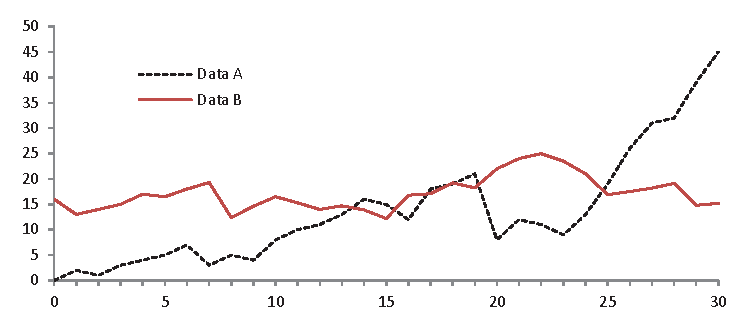
\includegraphics[width=\textwidth]{fig1.eps}
\caption{A figure caption is always placed below the illustration.
Please note that short captions are centered, while long ones are
justified by the macro package automatically.} \label{fig1}
\end{figure}

\begin{theorem}
This is a sample theorem. The run-in heading is set in bold, while
the following text appears in italics. Definitions, lemmas,
propositions, and corollaries are styled the same way.
\end{theorem}
%
% the environments 'definition', 'lemma', 'proposition', 'corollary',
% 'remark', and 'example' are defined in the LLNCS documentclass as well.
%
\begin{proof}
Proofs, examples, and remarks have the initial word in italics,
while the following text appears in normal font.
\end{proof}
For citations of references, we prefer the use of square brackets
and consecutive numbers. Citations using labels or the author/year
convention are also acceptable. The following bibliography provides
a sample reference list with entries for journal
articles~\cite{ref_article1}, an LNCS chapter~\cite{ref_lncs1}, a
book~\cite{ref_book1}, proceedings without editors~\cite{ref_proc1},
and a homepage~\cite{ref_url1}. Multiple citations are grouped
\cite{ref_article1,ref_lncs1,ref_book1},
\cite{ref_article1,ref_book1,ref_proc1,ref_url1}.
%
% ---- Bibliography ----
%
% BibTeX users should specify bibliography style 'splncs04'.
% References will then be sorted and formatted in the correct style.
%
% \bibliographystyle{splncs04}
% \bibliography{mybibliography}
%
\begin{thebibliography}{8}
\bibitem{ref_article1}
Author, F.: Article title. Journal \textbf{2}(5), 99--110 (2016)

\bibitem{ref_lncs1}
Author, F., Author, S.: Title of a proceedings paper. In: Editor,
F., Editor, S. (eds.) CONFERENCE 2016, LNCS, vol. 9999, pp. 1--13.
Springer, Heidelberg (2016). \doi{10.10007/1234567890}

\bibitem{ref_book1}
Author, F., Author, S., Author, T.: Book title. 2nd edn. Publisher,
Location (1999)

\bibitem{ref_proc1}
Author, A.-B.: Contribution title. In: 9th International Proceedings
on Proceedings, pp. 1--2. Publisher, Location (2010)

\bibitem{ref_url1}
LNCS Homepage, \url{http://www.springer.com/lncs}. Last accessed 4
Oct 2017
\end{thebibliography}
\end{document}
